%%%%%%%%%%%%%%%%%%%%%%%%%%%%%%%%%%%%%%%%%%%%%%%%%%%%%%%%%%%%%%%%%%%%%%%%%%%
%% Rulebook RoboCup Logisitc League
%% 2021 Challenges
%%%%%%%%%%%%%%%%%%%%%%%%%%%%%%%%%%%%%%%%%%%%%%%%%%%%%%%%%%%%%%%%%%%%%%%%%%%
% chktex-file 29
\documentclass[12pt,twoside]{article}
\usepackage[a4paper]{anysize}
\marginsize{2cm}{2cm}{1cm}{2cm}

\setlength{\marginparwidth}{1cm}
%\usepackage{fourier}

\usepackage{floatpag}
\usepackage{wrapfig}
\usepackage{fnpct}

\usepackage[table]{xcolor}

\usepackage[binary-units=true]{siunitx}
%% HYPERREF %%%%%%%%%%%%%%%%%%%
\usepackage{hyperref}
\hypersetup{
  pdftitle      = {The RoboCup Logistics League Challenge Rulebook for 2021},
  pdfauthor     = {RCLL TC},
  pdfkeywords   = {RCLL, Rulebook, Challenges},
  pdfsubject    = {},
  hidelinks,
}
\usepackage{tabularx}
\usepackage{multicol}
\usepackage{multirow}
\usepackage{calc}
\usepackage{float}
\usepackage{hhline}
\usepackage{longtable}

\restylefloat{table}
%% INPUTENC %%%%%%%%%%%%%%%%%%%
\usepackage{wasysym}
\usepackage[utf8]{inputenc}
\input{macros.tex}

\newcolumntype{C}{>{\raggedright\arraybackslash}X}

\newcommand{\refsec}[1]{Section~\ref{#1}}
\newcommand{\reffig}[1]{Figure~\ref{#1}}
\newcommand{\refdef}[1]{Definition~\ref{#1}}
%\newcommand{\reflst}[1]{Listing~\ref{#1}}
\newcommand{\reflst}[1]{Figure~\ref{#1}}
\newcommand{\reftab}[1]{Table~\ref{#1}}
\usepackage{acronym}
\acrodef{BS}{base station}
\acrodef{CS}{cap station}
\acrodef{RS}{ring station}
\acrodef{SS}{storage station}
\acrodef{DS}{delivery station}
\acrodef{MPS}{modular production system}
\acrodef{RCLL}{RoboCup Logistics Leaugue}
\acrodef{OC}{Organizational Committee}
\acrodef{TBD}{To be Discussed}

\usepackage{todonotes}
\presetkeys%
    {todonotes}%
    {inline}{}
\begin{document}
\begin{titlepage}
 \vspace*{5cm}
 \begin{center}
  \begin{LARGE}

   {\bf RoboCup Logistics League}\\[2ex]
   {\Large \bf{Challenges}}\\[4ex]
   {\Large Rules and Regulations 2021}\\[4ex]
  \end{LARGE}
  \hrule

  {\LARGE\vspace*{4ex}}
  \begin{Large}
   The Technical Committee 2012--2021\\[6ex]
  \end{Large}
  \begin{tabular}{lll}
   \textbf{Vincent Coelen}&\textbf{Christian Deppe}&\textbf{Till Hofmann}\\
	\textbf{Ulrich Karras}&\textbf{Peter Kohout}&\textbf{Alain Rohr}\\
	\textbf{Matthias Studer} &\textbf{Thomas Ulz}&\textbf{Tarik Viehmann}\\[.5em]
   Daniel Ewert&Nils Harder&S\"oren Jentzsch\\
   Nicolas Meier&Sebastian Reuter&Wataru Uemura\\
   Gerald Steinbauer&Tobias Neumann&Mostafa Gomaa\\
	 Tim Niemueller
  \end{tabular}
  \vfill
  Revision Date: 07.05.2021\\
 \end{center}
\end{titlepage}


\section{Introduction}
\label{sec:intro}
This additional rulebook aims to provide a competition in the RoboCup logistics
league domain, where the main tasks of the league are captured in isolated
challenges.
The objectives of this new competition are:
\begin{itemize}
 \item to provide a framework that allows teams to show and evaluate their
       progress in the individual tasks of the RCLL
 \item to ease the preparation for the main competition through providing a
       simplified cost- and space-efficient setup suitable for replication in
       local labs
 \item to be attractive for both RoboCup live events and online competitions,
       where teams can participate remotely from all over the world
\end{itemize}
This document is not self-sufficient, instead all the rules from the main
rulebook\footnote{\url{https://github.com/robocup-logistics/rcll-rulebook/releases}}
apply, unless stated otherwise.
The proposed format is carried out at RoboCup 2021, which is held remotely.
Hence the remainder of this document establishes the rules around the online
competition.

\section{Qualification}
\label{sec:qualification}
In addition to the regular Qualification process, teams have to participate
in a \href{https://fh-aachen.sciebo.de/s/Qkm7VfIIEIIJk1d}{RefBox workshop, see here}.
To complete the workshop, a game report dump of at least 2 Challenges
has to be submitted to the \acf{OC}.

\section{Requirements to score points}
\label{sec:scoring}
For your challenges to count as completed and score points you need to submit
the recorded video footage to the OC.
Further you need to submit your game reports from the MongoDB to the OC.
Your submission will not be counted if the footage shows human
interference with the field, machines or robots outside of
the specified rules in Section \ref{sec:operators}.

\section{Competition Area}
\subsection{Field Layout}
The competition area for the main challenges consists of a \SI{5 x 5}{\metre}
area divided in square zones of \SI{1 x 1}{\metre}. Additional challenges that
are not counting towards the scoring of the competition are carried out on
a \SI{7 x 8}{\metre} field instead (corresponding to halve the field of the
regular \ac{RCLL} field).
The field is a subset of the magenta-halve of the regular field as depicted
in \reffig{fig:challenge-field}.

\begin{figure}
	\centering
	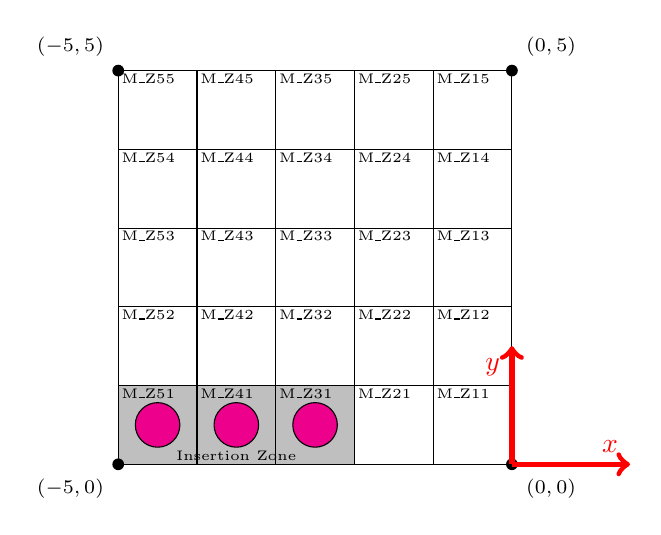
\begin{tikzpicture}[x=-1cm,y=1cm]
	\fill[gray!50!white] (2,0) rectangle (5,1);
	\node at (3.5,0) [anchor=south, font=\tiny, inner sep=1pt] {Insertion Zone};
	\foreach \i in {0,...,5} {
		\draw (0,\i) -- (5,\i);
		\draw (\i,0) -- (\i,5);
	}
	\foreach \i in {1,...,3} {
		\node at (1.5+\i,0.5) [circle,fill=magenta, draw=black,inner sep=0.2cm] {};
	}
	\foreach \x in {1,...,5} {
		\foreach \y in {1,...,5} {
			\node[font=\tiny,anchor=north west, inner sep=1pt] at (\x,\y) {M\_Z\x\y};
		}
	}
	\node at (0,0) [circle,fill,inner sep=1.5pt,label={[font=\scriptsize]-45:$(0,0)$}]{};
	\node at (5,0) [circle,fill,inner sep=1.5pt,label={[font=\scriptsize]225:$(-5,0)$}]{};
	\node at (5,5) [circle,fill,inner sep=1.5pt,label={[font=\scriptsize]135:$(-5,5)$}]{};
	\node at (0,5) [circle,fill,inner sep=1.5pt,label={[font=\scriptsize]45:$(0,5)$}]{};
	\draw[line width=2pt,red,->] (0,0) -- node[above left,pos=1] {$x$} (-1.5,0);
	\draw[line width=2pt,red,->] (0,0) -- node[below left,pos=1] {$y$} (0,1.5);
\end{tikzpicture}
	\caption{The \SI{5 x 5}{\metre} playing field.}
	\label{fig:challenge-field}
\end{figure}

The entire area belongs to a single team. The bottom left-most
\SI{1 x 3}{\metre} area is called the insertion zone and provides the starting
positions for up to three robots.
Contrary to the full RCLL field, it is not necessary to build partial walls
around the insertion zone and robots may be move freely in and out of the
insertion zone.
\subsection{Mockup Machines}\label{sec:machines}
In case no real \ac{MPS} stations are available, replications
(so called \emph{mockup machines}) may be used, that do not need to
physically perform the respective production steps. Instead, that work may
be carried out by a human supervisor (see \refsec{sec:operators}).
The minimum requirements for a mockup machine are specified in the following.

Mockup machines are required to have the same box-like base-shape as specified
in the RCLL rulebook.
Additionally, the following parts need to be mounted:
\begin{itemize}
	\item a model of the conveyor belt
	\item a shelf on the front right side of the box on stations replicating a \ac{CS}
	\item either a shelf, a slide or a conveyor belt on the front right side
of the box, such that it is accessible from the front on stations replicating a \ac{RS}
\end{itemize}
Models for a conveyor belt, shelf and slides can be found in the RCLL rulebook
repository\footnote{\url{https://github.com/robocup-logistics/rcll-rulebook/tree/common/challenges/mock_up_models}}.

The building materials for the models must be opaque, but may have any color.

In order to compete in all main challenges, a minimum number of 3 mockup
machines are required. On higher difficulty some challenges may require
4 mockup stations and some secondary challenges require 7 stations.

\subsection{Remote Setup}
In case a competition is carried out remotely, a proper local setup has to
be established and approved by the \ac{OC}.
Requirements include a proper camera setup that covers the field sufficiently,
such that external viewers can verify the integrity of each challenges,
as well as an approval for every mockup machine and robot that is used.
After registration the \ac{OC} will verify the field setup in a video call.
The validation call will be scheduled individually for each team
to account for timezones.

\section{Game Play}
\subsection{Competition Scope}
Each team can attempt a challenge by specifying a 30 minute time slot along
with the challenge in advance of the respective competition day.
The announcement procedure is managed by the \ac{OC}.
Each slot can be used to do at most one challenge and is split in two phases:
1. In the \texttt{SETUP} phase the participants ensure that
\begin{itemize}
	\item the video stream is setup via Zoom,
	\item the RefBox is started with the appropriate settings for the challenge,
	\item the machines and robots are placed on the field according to the rules
	\item and the robots are started.
\end{itemize}
The setup must be completed within 10 minutes, otherwise the attempt is counted
as a failure.
Then the \texttt{PRODUCTION} phase starts by instructing the RefBox accordingly.
During the production phase the team has 20 minutes to solve the challenge.

A team may retry the challenge by setting the RefBox back to the setup phase
and then starting the production phase again.
Only the last attempt in each slot can be counted. A team may decide to count
no attempt at all. Once a challenge is counted, it
may not be retried again, unless the difficulty is increased.
In order to complete an attempt, the RefBox needs to be set to phase
\texttt{POST\_GAME}.

All challenges are conducted while measuring the execution time of the
corresponding attempt, starting from the begin of the \texttt{PRODUCTION} phase
and ending at the begin of \texttt{POST\_GAME}.
The fastest team to complete a challenge on the selected difficulty gains $5$
additional points. A challenge is only completed if the full score is achieved,
so getting only partial credits for a challenge disqualifies from getting the
bonus points for the fastest completion.

\subsection{Changes compared to the Main Competition}
The tasks covered in the various challenges mostly obey the regular rules
for the \ac{RCLL}. However, some aspects are altered to simplify the setup.
The changes are not affecting existing machine communication and processing
steps, such that the challenges can be carried out on real machines as well as
on mockup versions obeying the requirements outlined in \refsec{sec:machines}.

\paragraph{Product Delivery}
The delivery procedure for finished products is altered compared to the
\ac{RCLL} rule set. In order to reduce the amount of machines required
for participation, Deliveries are made by bringing the finished product
to the insertion zone and dropping it there.

\paragraph{Ring Payments}
Easing the setup of mockup machines, it is not required to have a slide
on ring stations. Instead, a shelf or additional conveyor may be mounted on the
machine to place payments at the corresponding station.

\paragraph{Ring Color Assignment}
The cost for mounting each ring color are fixed, the assignment of ring colors
is semi-fixed as teams can choose between two different options for each
challenge (\texttt{option1} or \texttt{option2} according to
\reftab{tab:ring-costs}).
The RefBox settings default to \texttt{option1}, but teams may change this
accordingly.

\newcommand{\colconfig}{\mathcal{RC}}
\begin{table}[!htb]
 \centering
 \begin{tabular}{l|l|l||l|l||l|l}
  & \multicolumn{4}{c||}{Ring Costs}
  & \multicolumn{2}{c}{\multirow{2}{*}{Color Assignment }}\\\cline{2-5}
  & Color  & Price & Color  & Price & \multicolumn{2}{c}{}\\\cline{2-7}
  & Yellow & 0 & Green & 0
  & RS1: $\colconfig_1$ & RS1: $\colconfig_2$ \\
  & Blue  & 1 & Orange & 2
  & RS2: $\colconfig_2$ & RS2: $\colconfig_1$ \\\hline\hline
  Configuration & \multicolumn{2}{c||}{$\colconfig_1$}
  & \multicolumn{2}{c||}{$\colconfig_2$}
  & $\texttt{option1}$ & $\texttt{option2}$\\
 \end{tabular}
 \caption{Materials}
 \label{tab:ring-costs}
\end{table}

\paragraph{Materials}\label{sec:materials}
The available material that can be used per challenge is restricted
(unless stated otherwise) per machine according to the information in
\reftab{tab:materials}.
\begin{table}[!htb]
 \centering
  \begin{tabularx}{\linewidth}{l|l}
   Machine & Available Material  \\\hline
   \ac{BS} & 2 bases of each color \\
   \ac{CS} & 3 cap-carriers (cap color choices up to each team)  \\
   \ac{RS} & 4 rings of each assigned color (8 in total)  \\
  \end{tabularx}
 \caption{Materials}
 \label{tab:materials}
\end{table}

\paragraph{Orders}
Unless specified otherwise, orders that have to be fulfilled in challenges
are entered through the web shop
(see the RefBox workshop in \refsec{sec:qualification})
by any member of the competing team.

In challenges where only one \ac{RS} is present, teams are responsible to
order products which can be assembled using the available stations only.

\paragraph{Scoring}\label{sec:scoring}
While the RefBox may assign points during challenges according to the
regular RCLL rules, those points do not count towards this competition.
Instead, the point scoring for each challenge is listed in
\refsec{sec:challenges}.

\subsection{Field Operators}\label{sec:operators}
In challenges where mockup machines are used, the actual assembly steps have
to be performed by human supervisors. Whenever a machine is instructed,
the RefBox operator announces the required interaction. One field operator may
proceed to enter the field in order to perform the interaction. Afterwards the
field has to be left immediately.
The usual rules for replenishing resources (respecting the limited materials
\refsec{sec:materials}) apply.

\subsection{Available Challenges for the Primary Competition}
\label{sec:challenges}
Challenges have different types and variations (difficulty levels).
The overall score of the competition is calculated by summing up the score
in the highest difficulty achieved in each of the challenge types.
The challenge types of the competition are described in
\refsec{sec:challenge-navigation}-\ref{sec:challenge-markerless}.

The RefBox is used to log the progress and data for each challenge.
Participating teams are required to send the corresponding game-report dumps
to the \ac{OC}.
Once the competition is finished, $5$ bonus points are awarded each time a
team solved a challenge on a difficulty in the shortest amount of time.

\subsubsection{Navigation Challenge}\label{sec:challenge-navigation}
Basic navigation task with known obstacles.\\
\textbf{Task:} Drive to 12 randomly generated target zones. A target zone is
reached, if any robot remains in that zone for at least 5 consecutive seconds.
The pose of each robot must be set in the beacon message
for the RefBox to properly register the zones as visited. The robot may move
within the zone during the 5 second period.\\
Variations of this challenge depend on the number of available machines
(see \reftab{tab:challenge-navigation}).
Multiple robots may be used to simultaneously to reach multiple target zones.
Partial points may be awarded in case only a subset of target zones were
reached, which are accumulated if the challenge is completed fully.

\begin{table}[!htb]
 \centering
 \begin{tabular}{l|l|l|l|l}
  \multirow{2}{*}{Machines}
  & \multicolumn{4}{c}{Scoring} \\\cline{2-5}
	& $\geq$ 4 zones  & $\geq$ 8 zones & all 12 zones  & combined \\\hline\hline
	 2 & +2 & +4 & +9 & 15 \\
	 3 & +3 & +6 & +14 & 23 \\
	 4 & +4 & +8 & +18 & 30 \\
 \end{tabular}
 \caption{Navigation Challenge}
 \label{tab:challenge-navigation}
\end{table}

\subsubsection{Exploration Challenge}\label{sec:challenge-exploration}
Replicate the RCLL exploration phase.
Machine Marker detection as well as navigational skills are required to solve
this challenge.\\
\textbf{Task:} Find and report all machines on the field (type and orientation)
according to the rules of a regular exploration phase.
\\
Variable in the number of machines
(see \reftab{tab:challenge-exploration}).
\begin{table}[!htb]
 \centering
 \begin{tabular}{l|l}
  Machines & Scoring \\\hline
  2   & 10 \\
  3   & 20 \\
  4   & 30 \\
 \end{tabular}
 \caption{Exploration Challenge}
 \label{tab:challenge-exploration}
\end{table}
This challenge needs to be run by setting the RefBox to phase
\texttt{EXPLORATION}.

\subsubsection{Grasping Challenge}\label{sec:challenge-grasping}
Simple grasping task.
Each Machine has a base at output.
Robots start at the zone in front of a machine output.\\
\textbf{Task:} A robot brings a base from one machine's output back to it's
input. A human supervisor places it back to the output. Repeat until all
products were placed at the respective machines input 3 times and all robots
returned to their starting positions. \\
Variations differ by number of machines, see
\reftab{tab:challenge-grasping}. The $i$-th repetition is considered to be
successful, once all bases were placed at the respective machine input
at least $i$ times.
The placement of the machines on the field is fixed according to
\reffig{fig:grasping-field}.

\begin{table}[!htb]
\centering
 \begin{tabular}{l|l|l}
  \multirow{2}{*}{Machines}
  & \multicolumn{2}{c}{Scoring} \\\cline{2-3}
  & first repetition
  & each subsequent repetiton  \\\hline\hline
  1 & +10 & +2 \\
  2 & +20 & +2 \\
  3 & +25 & +2 \\
 \end{tabular}
 \caption{Grasping Challenge}
 \label{tab:challenge-grasping}
\end{table}

\begin{figure}
	\centering
	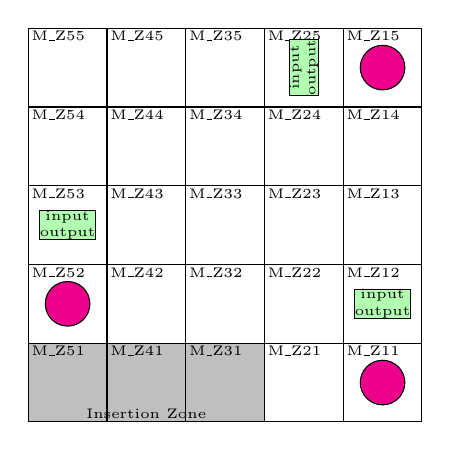
\begin{tikzpicture}[x=-1cm,y=1cm]
	\fill[gray!50!white] (2,0) rectangle (5,1);
	\node at (3.5,0) [anchor=south, font=\tiny, inner sep=1pt] {Insertion Zone};
	\foreach \i in {0,...,5} {
		\draw (0,\i) -- (5,\i);
		\draw (\i,0) -- (\i,5);
	}
	\foreach \x in {1,...,5} {
		\foreach \y in {1,...,5} {
			\node[font=\tiny,anchor=north west, inner sep=1pt] at (\x,\y) {M\_Z\x\y};
		}
	}
		\node at (4.5,1.5) [circle,fill=magenta, draw=black,inner sep=0.2cm] {};
		\node at (4.5,2.5) [rectangle,fill=green!30!white, draw=black,inner sep=0.1pt,align=center,font=\tiny] {input\\output};
		\node at (0.5,0.5) [circle,fill=magenta, draw=black,inner sep=0.2cm] {};
		\node at (0.5,1.5) [rectangle,fill=green!30!white, draw=black,inner sep=0.1pt,align=center,font=\tiny] {input\\output};
		\node at (0.5,4.5) [circle,fill=magenta, draw=black,inner sep=0.2cm] {};
		\node at (1.5,4.5) [rectangle,fill=green!30!white, draw=black,inner sep=0.1pt,align=center,font=\tiny,rotate=90] {input\\output};

\end{tikzpicture}
\caption{Starting configuration for the grasping challenge.
	BS is placed at $\texttt{M\_Z12}$, CS1 is placed at $\texttt{M\_Z53}$
and RS1 is placed at $\texttt{M\_Z25}$.}
	\label{fig:grasping-field}
\end{figure}

\subsubsection{Product Challenges}\label{sec:challenge-cx}
This section covers four types of challenges, which all can be individually
completed.
Each challenge corresponds to the production of a product with one of the
available complexities (C0, C1, C2, C3) in the \ac{RCLL} using either
one or two \ac{RS}.\\
For complexities C1, C2 and C3 the accumulated cost for mounting the required
rings must be equal to 1, 2 and 3, respectively.
\textbf{Task:} Produce all posted orders.\\
\begin{table}[!htb]
 \centering
 \begin{tabular}{l|l|l}
  Machines & Challenge type & Scoring \\\hline
  2 & C0 & 30 \\
  3 & C1 & 50 \\
  4 & C1 & 50 \\
  3 & C2 & 70 \\
  4 & C2 & 70 \\
  3 & C3 & 100 \\
  4 & C3 & 100 \\
 \end{tabular}
 \caption{CX Challenge}
 \label{tab:challenge-cx}
\end{table}

\subsubsection{Exploration + C0 Challenge}\label{sec:challenge-combine-exp-c0}
A simple production task on a field with unknown machine positions.
The challenge is to produce a product of complexity C0 without receiving the
machine positions at the start of the production phase, resembling a unified
exploration and production phase.\\
\textbf{Task:} Produce all posted orders.\\
Beating this challenges yields 50 points.

%\subsubsection{RefBox Simulation Challenge}\label{sec:challenge-simulation}
%A competition on the agent level. The RefBox provides a set of actions
%that can be executed by sending dedicated commands to the RefBox via protobuf.
%Hence no actual robot is required to participate.
%\textbf{Task:} Play a regular RCLL game through the RefBox simulation
%interface.\\
%Participating in this challenge yields points based on the achieved in-game
%points, see \reftab{tab:challenge-simulation}.
%Additionally, the team scoring the highest points overall gets awarded another
%$10$ points
%\begin{table}[!htb]
% \centering
% \begin{tabular}{l|l|l|l}
%  Points & Scoring \\\hline
%  $[0,50)$ & 0\\% chktex 9
%  $[50,150)$ & 20\\% chktex 9
%  $[150,250)$ & 40 \\% chktex 9
%  $[250,\infty)$ & 60 \\% chktex 9
% \end{tabular}
% \caption{CX Challenge}
% \label{tab:challenge-cx}
%\end{table}


\subsubsection{Markerless Detection Challenge}\label{sec:markerless}
Image recognition challenge to classify different machine types.\\
\textbf{Task:} Autonomously label the machines shown in a set of pictures
by their type.
A picture may contain more than one machine, which all count towards the
total number of machines to detect.\\
As a preparation for this challenge, a data set will be supplied to
all participants which may be used for training and testing purposes
\footnote{\url{https://fh-aachen.sciebo.de/s/MRghypMQSMhTYaC}}.
The evaluation set for the challenge consists of a set of separate images.
\begin{table}[!htb]
 \centering
 \begin{tabularx}{\linewidth}{l|l|l|l}
  \% Correctly Classified & \% Wrongly Classified & \% Not Classified
  & Scoring \\\hline
  $x$ & $y$ & $z$ & $(x-y)\cdot30$
 \end{tabularx}
 \caption{Machine Detection Challenge}
 \label{tab:challenge-markerless}
\end{table}

\subsection{Challenges for the Secondary Competition}

\subsubsection{Full game}\label{sec:challenge-full-game}
Play a full RCLL game on a field of \SI{7 x 8}{\metre} with $7$ machines
(no machines from the opposing team). The normal RCLL rules apply.
\subsubsection{Full game}\label{sec:challenge-full-game}
Play the production phase of an RCLL game on a field of \SI{7 x 8}{\metre} with
$7$ machines (no machines from the opposing team).
The normal RCLL rules apply with the exception that the ground truth for
machine positions is not sent by the RefBox.
\end{document} %chktex 17
